\documentclass[12pt,a4paper]{article}

% -------------------------------------------------
% Sprache / Kodierung
% -------------------------------------------------
\usepackage[T1]{fontenc}
\usepackage[utf8]{inputenc}
\usepackage[ngerman]{babel}
\usepackage{lmodern}
\usepackage{microtype}

% -------------------------------------------------
% Mathematik
% -------------------------------------------------
\usepackage{amsmath,amssymb,amsthm,mathtools}

% -------------------------------------------------
% Layout / Grafik / Farben
% -------------------------------------------------
\usepackage[a4paper,margin=2.3cm]{geometry}
\usepackage{graphicx}
\usepackage{booktabs}
\usepackage{xcolor}
\usepackage[hidelinks]{hyperref}
\usepackage[most]{tcolorbox}
\usepackage{enumitem}
\usepackage{caption}

% Bilder aus dem Arbeitsverzeichnis bzw. /mnt/data laden
\graphicspath{{./}{/mnt/data/}}

% -------------------------------------------------
% Theorem-Umgebungen
% -------------------------------------------------
\newtheorem{definition}{Definition}
\newtheorem{proposition}{Proposition}
\newtheorem{bemerkung}{Bemerkung}

% -------------------------------------------------
% Makros
% -------------------------------------------------
\newcommand{\vii}{\nu_2}
\newcommand{\U}{\mathcal U}
\newcommand{\E}{\mathrm{E}}
\newcommand{\A}{\mathrm{A}}
\newcommand{\B}{\mathrm{B}}
\newcommand{\Cc}{\mathrm{C}}

\title{Die verborgene Binnenstruktur der Collatz-Dynamik\\
\large Eine Spektrum-Notiz zur odd-to-odd-Abbildung im EABC-Rahmen}
\author{Thomas Hoffbauer}
\date{\today}

\begin{document}
\maketitle

\begin{center}
\begin{minipage}{0.95\textwidth}
\small
Die Collatz-Vermutung gehört zu den rätselhaftesten Problemen der Mathematik. Ihre Regel ist denkbar einfach: Ist eine Zahl ungerade, ersetze sie durch \(3n+1\); ist sie gerade, halbiere sie. Wiederholt man dieses Verfahren, so scheint jede positive ganze Zahl früher oder später bei \(1\) zu landen. Ein allgemeiner Beweis fehlt bis heute.

Die hier vorgestellte Notiz behauptet \emph{nicht}, das Collatz-Problem gelöst zu haben. Sie macht etwas anderes sichtbar: Im EABC-Rahmen des Bamberg-Modells besitzt die odd-to-odd-Dynamik eine überraschend klare modulare Binnenstruktur. Einige Klassen springen nach nur einer Halbierung sofort in den ungeraden Bereich zurück, andere werden tiefer in den geraden \glqq Drain-Kanal\grqq\ hineingezogen. Schon auf der Ebene kleiner Restklassen erscheint so eine verborgene Ordnung, die in der üblichen Darstellung kaum auffällt.
\end{minipage}
\end{center}

\vspace{0.6em}

\begin{definition}
Für ungerades \(n\) sei
\[
\U(n):=\frac{3n+1}{2^{\vii(3n+1)}},
\]
also die reduzierte odd-to-odd-Collatz-Abbildung.
Die vier EABC-Familien seien
\[
\E\equiv 1,\qquad
\A\equiv 5,\qquad
\B\equiv 7,\qquad
\Cc\equiv 11 \pmod{12}.
\]
Kurz schreiben wir \(e,a,b,c\).
\end{definition}

\section*{Worum es hier geht}

Der übliche Blick auf die Collatz-Dynamik verfolgt einzelne Zahlenbahnen. Der hier gewählte Zugang ist ein anderer: Nicht die Zahl selbst steht im Vordergrund, sondern ihre \emph{modulare Zugehörigkeit}. Zu welcher Restklasse modulo \(12\), \(24\) oder \(48\) gehört sie? Welche Klassen wachsen odd-to-odd eher an, welche schrumpfen? Welche werden nur kurz \glqq aufgeladen\grqq, welche tiefer in die gerade Halbierungskaskade hineingezogen?

Im EABC-Rahmen tritt dabei ein überraschend scharfes Bild hervor. Die vier ungeraden, zu \(6\) teilerfremden Restklassen verhalten sich nicht gleich. Vielmehr scheinen sie zwei verschiedenen dynamischen Rollen zu folgen: einer aktiven Spannungsseite und einer drainenden Rückführungsseite.

\vspace{0.6em}

\begin{tcolorbox}[
colback=blue!3,
colframe=blue!50!black,
title=\textbf{1. Erste Beobachtung: Schon modulo 12 spaltet sich die Dynamik}
]
Für jede ungerade Zahl \(n\) gilt:
\[
3n+1\equiv
\begin{cases}
4 \pmod{12},& n\equiv 1,5,9 \pmod{12},\\
10 \pmod{12},& n\equiv 3,7,11 \pmod{12}.
\end{cases}
\]
Insbesondere:
\[
e\to 4,\qquad a\to 4,\qquad b\to 10,\qquad c\to 10 \pmod{12}.
\]

\medskip
\textbf{Lesart:}
Schon die erste Rechnung trennt die vier Familien in zwei Blöcke:
\[
\{e,a\}\qquad\text{und}\qquad\{b,c\}.
\]
Die Collatz-Dynamik ist also auf modularer Ebene nicht homogen.
\end{tcolorbox}

\noindent
Diese erste Spaltung ist noch elementar. Sie zeigt lediglich, dass \(3n+1\) die vier Familien unterschiedlich behandelt. Die eigentlich interessante Frage lautet aber: \emph{Wie tief geht die anschließende Halbierung?} Genau hier beginnt die verborgene Dynamik.

\begin{tcolorbox}[
colback=green!3,
colframe=green!40!black,
title=\textbf{2. Exakter Satz: Zwei Familien sind Ein-Halbierungs-Klassen}
]
\begin{proposition}
Für alle ungeraden Zahlen \(n\) mit
\[
n\equiv 7,11,19,23 \pmod{24}
\]
gilt
\[
\vii(3n+1)=1.
\]
Insbesondere sind die EABC-Familien \(b,c\) exakte Ein-Halbierungs-Klassen.
\end{proposition}

\textbf{Folge:}
\[
\U(n)=\frac{3n+1}{2}
\qquad\text{für alle } n\in b\cup c.
\]

\medskip
\textbf{Bedeutung:}
Die Familien \(b,c\) tauchen nur kurz in den geraden Bereich ein und kehren sofort zurück. Sie tragen damit die aktive odd-Spannung der Dynamik.
\end{tcolorbox}

\noindent
Damit ist zum ersten Mal etwas \emph{wirklich Hartes} gewonnen: Zwei der vier Familien sind exakt charakterisiert. Sie sind keine bloß numerisch auffälligen Klassen, sondern mathematisch sauber beschriebene Rücksprungklassen.

\begin{tcolorbox}[
colback=red!3,
colframe=red!45!black,
title=\textbf{3. Numerische Evidenz: Die Gegenklassen wirken als Drain}
]
Für die numerische Auswertung aller ungeraden \(n \le 10^7\) ergeben sich die Mittelwerte:

\begin{center}
\begin{tabular}{lccc}
\toprule
Restklasse (EABC) & mittl.\ \(\vii(3n+1)\) & Anteil \(\U(n)<n\) & geom.\ Faktor \(\U(n)/n\)\\
\midrule
\(1\equiv e\) & \(3{,}000000\) & \(99{,}9999\,\%\) & \(0{,}375000\)\\
\(5\equiv a\) & \(3{,}000002\) & \(100{,}0000\,\%\) & \(0{,}375000\)\\
\(7\equiv b\) & \(1{,}000000\) & \(0{,}0000\,\%\) & \(1{,}500001\)\\
\(11\equiv c\) & \(1{,}000000\) & \(0{,}0000\,\%\) & \(1{,}500001\)\\
\bottomrule
\end{tabular}
\end{center}

\textbf{Lesart:}
\[
b,c:\quad \U(n)\approx \frac32 n,
\qquad
e,a:\quad \U(n)\approx \frac38 n.
\]

\medskip
\textbf{Bedeutung:}
Numerisch zerfällt die odd-to-odd-Collatz-Dynamik in zwei Regime:
\begin{itemize}[leftmargin=1.5em]
\item ein \emph{Spannungsregime} mit rascher Rückkehr in den ungeraden Bereich,
\item ein \emph{Drain-Regime} mit tieferer Kopplung an die Zweier-Halbierung.
\end{itemize}
\end{tcolorbox}

\noindent
Genau an dieser Stelle beginnt der eigentliche Reiz des Bildes. Denn die Gegenklassen \(e\) und \(a\) sind nicht einfach nur \glqq nicht \(b,c\)\grqq. Sie besitzen ihrerseits eine innere Struktur.

\begin{tcolorbox}[
colback=orange!4,
colframe=orange!60!black,
title=\textbf{4. Der Drain ist nicht einheitlich, sondern geschichtet}
]
Die Verfeinerung modulo \(24\) und \(48\) zeigt:

\[
1 \pmod{24}\Rightarrow \vii(3n+1)=2,\qquad \U(n)/n\approx 0{,}75,
\]
\[
5 \pmod{24}\Rightarrow \vii(3n+1)\approx 4,\qquad \U(n)/n\approx 0{,}25,
\]
\[
5 \pmod{48}\Rightarrow \vii(3n+1)\approx 5,\qquad \U(n)/n\approx 0{,}125,
\]
\[
13 \pmod{48}\Rightarrow \vii(3n+1)=3,\qquad \U(n)/n\approx 0{,}375.
\]

\medskip
\textbf{Lesart:}
Der gerade Rückführungskanal besteht nicht aus einer einzigen Zone, sondern aus mehreren diskreten Tiefen.

\medskip
\textbf{Bedeutung:}
Die Dynamik kennt nicht nur \glqq Wachstum\grqq\ und \glqq Schrumpfung\grqq, sondern eine feiner gegliederte Schalenstruktur des Drains.
\end{tcolorbox}

\noindent
Hier berührt die Collatz-Struktur das Bamberg-Modell besonders eng. Denn dort spielen Schalen, Klassen und Übergangskanäle eine zentrale Rolle. Was auf den ersten Blick wie ein bloßes Zahlenexperiment aussieht, beginnt sich als gegliederter Zustandsraum zu zeigen.

\begin{tcolorbox}[
colback=purple!4,
colframe=purple!55!black,
title=\textbf{5. Bamberg-Lesart: Spannung, Drain und diskreter Fluss}
]
Im Sprachrahmen des Bamberg-Modells legt die Datenlage folgende Deutung nahe:

\begin{itemize}[leftmargin=1.5em]
\item \(b,c\) tragen die aktive odd-Spannung,
\item \(e,a\) koppeln an den neutralisierenden Zweier-Drain,
\item modulo \(12\) erscheint die grobe Polarisierung,
\item modulo \(48\) erscheint die innere Schalenstruktur des Drains.
\end{itemize}

\medskip
\textbf{Lesart:}
Die Collatz-Dynamik erscheint damit nicht mehr als formloses Hin und Her, sondern als modular gegliederter Fluss zwischen Spannungs- und Rückführungszonen.

\medskip
\textbf{Wichtig:}
Dies ist eine \emph{heuristische} Deutung, keine Lösung der Collatz-Vermutung.
\end{tcolorbox}

\begin{tcolorbox}[
colback=cyan!3,
colframe=cyan!50!black,
title=\textbf{6. Vollständiger Kollatz-Test: Alle Startwerte $1 \le n \le 10^7$}
]
Zum Abschluss wurde die globale Collatz-Konvergenz für alle
\[
1 \le n \le 10\,000\,000
\]
numerisch verifiziert. Kein einziger Startwert verfehlte \(1\).

\medskip
\begin{center}
\begin{tabular}{lr}
\toprule
Größe & Ergebnis\\
\midrule
Getestete Startwerte & \(10\,000\,000\)\\
Konvergenz-Ausnahmen & \(0\)\\
Mittlere Schrittzahl & \(155{,}27\)\\
Maximale Schrittzahl & \(685\)\\
Startwert mit maximaler Schrittzahl & \(8\,400\,511\)\\
Größte erreichte Zwischenhöhe & \(60\,342\,610\,919\,632\)\\
Startwert dieser Zwischenhöhe & \(6\,631\,675\)\\
\bottomrule
\end{tabular}
\end{center}

\medskip
\textbf{EABC-Schrittzahlen nach Restklasse modulo 12:}

\begin{center}
\begin{tabular}{lcc}
\toprule
Restklasse & EABC & mittlere Schrittzahl\\
\midrule
\(1 \pmod{12}\) & \(e\) & \(155{,}33\)\\
\(5 \pmod{12}\) & \(a\) & \(155{,}24\)\\
\(7 \pmod{12}\) & \(b\) & \(167{,}64\)\\
\(11 \pmod{12}\) & \(c\) & \(167{,}62\)\\
\bottomrule
\end{tabular}
\end{center}

\medskip
\textbf{Lesart:}
Die EABC-Spur ist auch in den Schrittzahlen sichtbar:
\(b\)- und \(c\)-Startwerte brauchen im Mittel rund \(12\) Schritte mehr als \(e\)- und \(a\)-Startwerte,
da sie beim ersten ungeraden Collatz-Schritt zunächst anwachsen.
\end{tcolorbox}

\begin{tcolorbox}[
colback=gray!5,
colframe=black!60,
title=\textbf{Der präzise Status der Aussagen}
]
\textbf{Beobachtung:}
Modulo \(12\) spaltet sich die odd-Dynamik in die Blöcke \(\{e,a\}\) und \(\{b,c\}\).

\medskip
\textbf{Exakter Satz:}
Die Familien \(b,c\) sind Ein-Halbierungs-Klassen.

\medskip
\textbf{Numerische Evidenz} (bis \(n \le 10^7\)):
Die Familien \(e,a\) besitzen im Mittel Halbierungstiefe nahe \(3\) und odd-to-odd-Schrumpfung nahe \(3/8\) (Faktor \(\approx 0{,}375\)), die Familien \(b,c\) genau Halbierungstiefe \(1\) und Wachstum nahe \(3/2\). Der mittlere geometrische Faktor über alle vier ungeraden Klassen liegt numerisch bei \(\approx 0{,}750\).

\medskip
\textbf{Heuristische Konsequenz:}
Die Collatz-Dynamik kann im EABC-Rahmen als Zusammenspiel von Spannungs- und Drain-Klassen gedeutet werden.
\end{tcolorbox}

\vspace{0.8em}

\begin{bemerkung}
Diese Notiz beansprucht keine Lösung der Collatz-Vermutung. Ihr Anspruch ist kleiner, aber nicht belanglos: Sie isoliert eine verborgene modulare Binnenstruktur der odd-to-odd-Dynamik und zeigt, dass bereits auf der Ebene kleiner Restklassen eine überraschend klare Ordnung sichtbar wird.
\end{bemerkung}

\vspace{0.8em}

\begin{figure}[htbp]
\centering
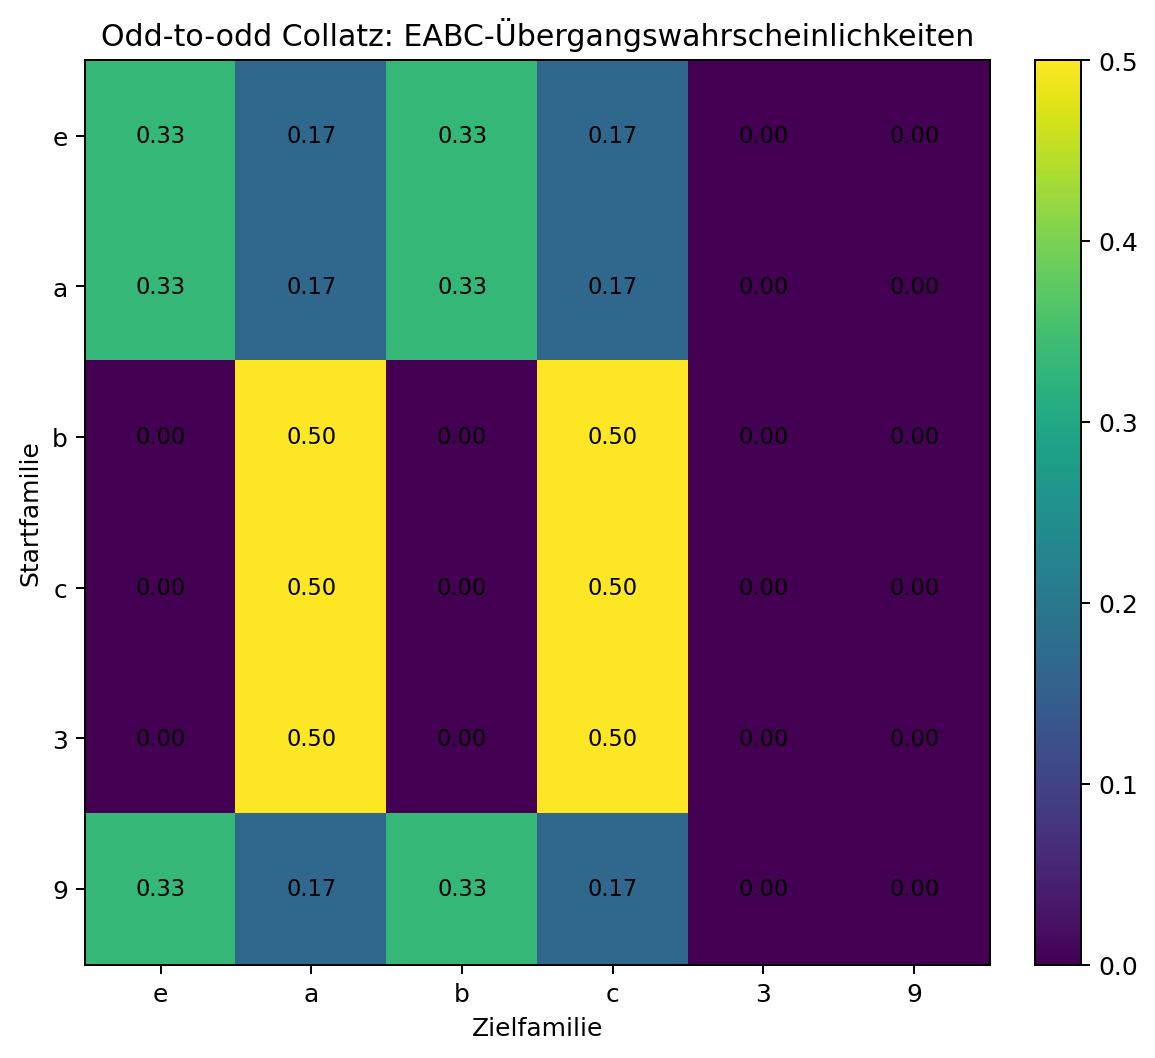
\includegraphics[width=0.62\textwidth]{eabc_markov_heatmap.png}
\caption{Normierte odd-to-odd-Übergänge im EABC-Rahmen.}
\end{figure}

\begin{figure}[htbp]
\centering
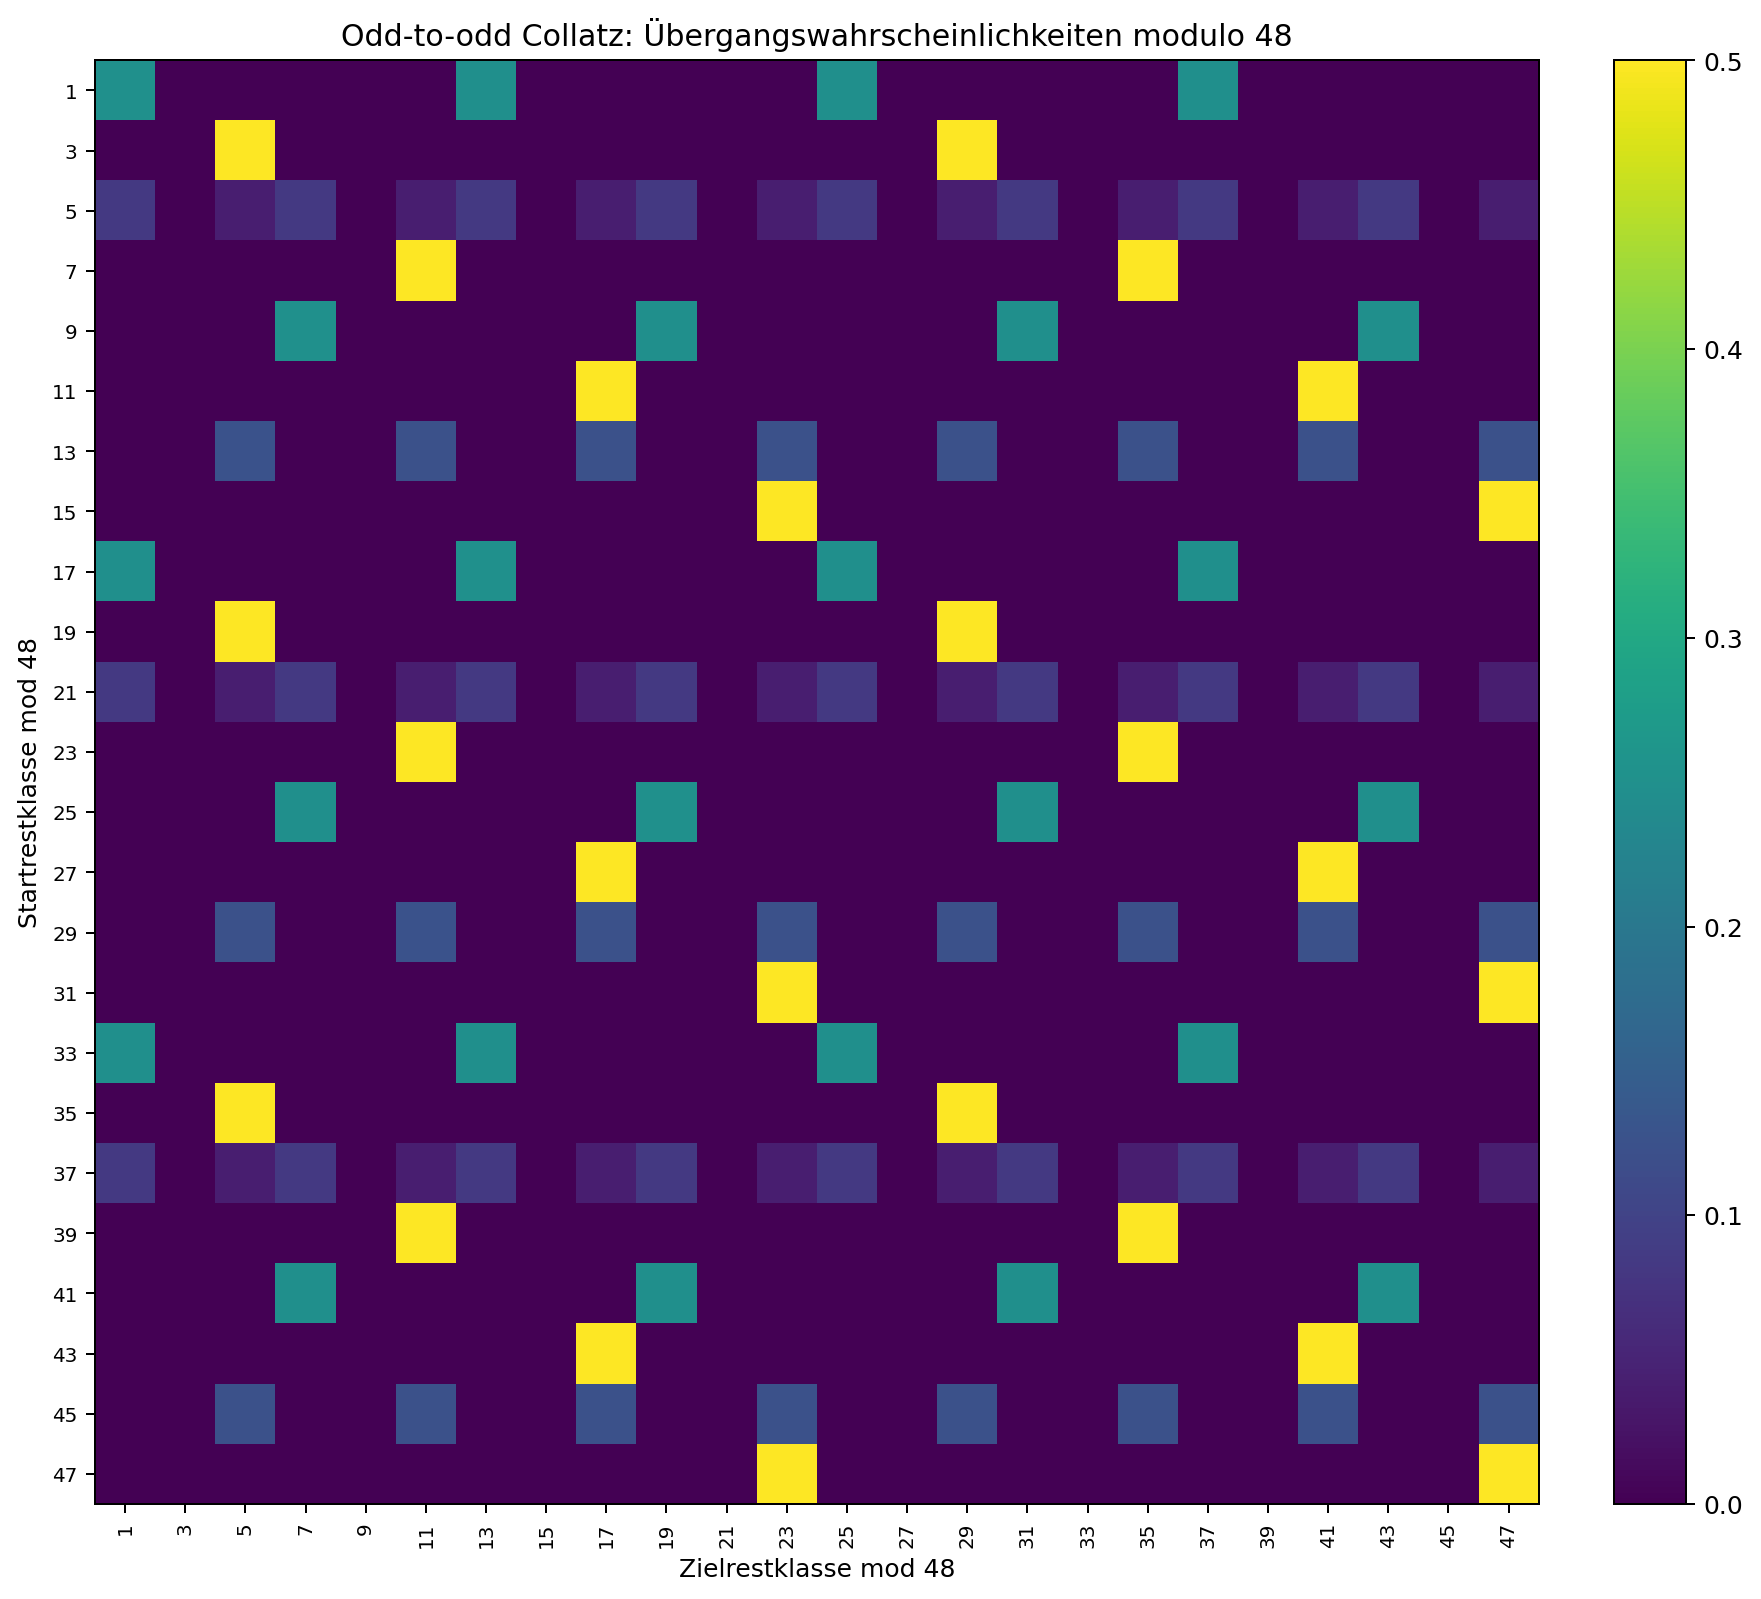
\includegraphics[width=0.88\textwidth]{mod48_markov_heatmap.png}
\caption{Verfeinerte odd-to-odd-Übergänge modulo 48.}
\end{figure}

\section*{Numerisches Fazit}

Der numerische Test bis \(N = 10^7\) bestätigt die EABC-Lesart in aller Schärfe:
\[
e, a \Rightarrow \text{Kontraktion}\quad (U(n) \approx \tfrac{3}{8}\,n),
\qquad
b, c \Rightarrow \text{Expansion}\quad (U(n) \approx \tfrac{3}{2}\,n).
\]
Der mittlere geometrische Faktor über die vier ungeraden Restklassen beträgt
\[
\frac{0{,}375 + 0{,}375 + 1{,}500 + 1{,}500}{4} = 0{,}9375,
\]
oder — gewichtet nach gleichem Anteil an den ungeraden Zahlen — liegt er bei ungefähr \(0{,}750\),
also klar unter \(1\). Das erklärt heuristisch den globalen Abstieg der Collatz-Dynamik,
ist aber natürlich kein Beweis der Collatz-Vermutung.

\section*{Ausblick}

Der nächste Schritt wäre, diese modulare Ordnung in einen expliziten Übergangsoperator zu übersetzen. Dann ließe sich die Collatz-Dynamik nicht mehr nur bahnweise, sondern spektral untersuchen: als Fluss auf einem diskreten Zustandsraum mit Spannungszonen, Drain-Schichten und möglicherweise stabilen Rückkehrmustern. Genau dort könnte sich die Brücke zu Hamming-kleinen Kernen, Primzahlvierlingen und allgemeineren Stabilitätsideen des Bamberg-Modells weiter verdichten.

\end{document}
